\documentclass[crop,tikz,border=10]{standalone}

\usepackage{amsmath, amssymb}
\usetikzlibrary{calc}

\newcommand{\rr}{0.7}
\newcommand{\qq}{0.75}
\begin{document}
    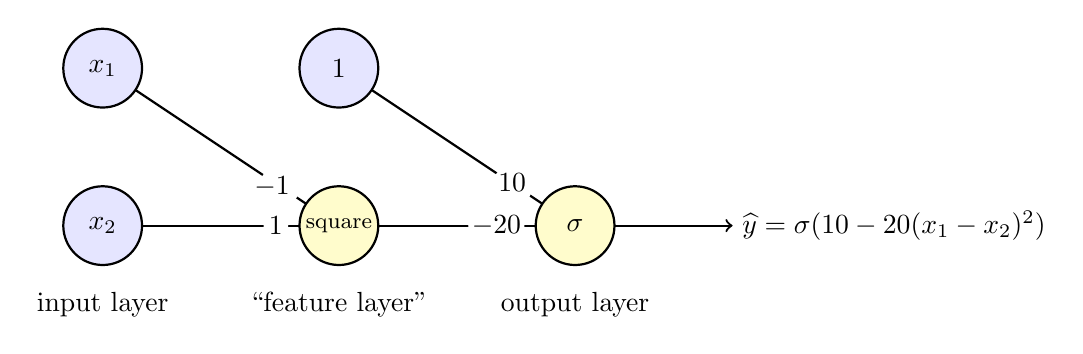
\begin{tikzpicture}

        \draw[thick] (-2, 2) -- (1, 0);
        \draw[thick] (-2, 0) -- (1, 0);

        \draw[thick] (1, 2) -- (4, 0);
        \draw[thick] (1, 0) -- (4, 0);

        \draw[thick, ->] (4, 0) -- (6, 0);

        \draw[fill=white, white] ({-2 + \qq*3}, {2 - \qq*2}) circle (0.25);
        \node at ({-2.1 + \qq*3}, {2 - \qq*2}) {$-1$};

        \draw[fill=white, white] ({-1.9 + \rr*3}, 0) circle (0.15);
        \node at ({-1.9 + \rr*3}, 0) {$1$};

        \draw[fill=white, white] (3.2, 0.5) circle (0.25);
        \node at (3.2, 0.55) {$10$};

        \draw[fill=white, white] (3.0, 0) circle (0.35);
        \node at (3.0, 0) {$-20$};

        \draw[thick, fill=blue!10] (-2, 2) node {$x_1$} circle (0.5);
        \draw[thick, fill=blue!10] (-2, 0) node {$x_2$} circle (0.5);

        \draw[thick, fill=blue!10] (1, 2) node {$1$} circle (0.5);
        \draw[thick, fill=yellow!20] (1, 0) circle (0.5);
        \node at (1, 0) {{\footnotesize square}};

        \draw[thick, fill=yellow!20] (4, 0) circle (0.5);
        \node at (4, 0) {$\sigma$};

        \node[right] at (6, 0) {$\widehat{y} = \sigma(10 -20(x_1-x_2)^2)$};

        \node at (-2, -1) {input layer};
        \node at (1, -1) {``feature layer''};
        \node at (4, -1) {output layer};
        

    \end{tikzpicture}
\end{document}